\pdfoptionpdfminorversion=5
\documentclass[spanish,professionalfonts]{beamer}
\usepackage{lmodern}
\usepackage[utf8]{inputenc}
\usepackage[spanish,mexico]{babel}
\usepackage{amsmath}
\usepackage{amssymb}
\usepackage{color}
\usepackage{xmpmulti}
\usefonttheme[onlymath]{serif}
\usepackage{tabularx}
\usepackage{listings}
%%Regular colours! 
\definecolor{MyBlack}{RGB}{0,0,0}
\definecolor{MyRed}{RGB}{255,0,0}
\definecolor{MyBlue}{RGB}{0,0,255}
\definecolor{MyGreen}{RGB}{0,200,0}
\definecolor{MyBrown}{RGB}{130,70,0}
\definecolor{MyPurple}{RGB}{120,0,160}
\definecolor{MyDarkPurple}{RGB}{100,0,140}
\definecolor{MyLightPurple}{RGB}{190,0,220}
\definecolor{MyYellow}{RGB}{190,190,0}
\definecolor{MyOrange}{RGB}{200,100,0}
\definecolor{MyCyan}{RGB}{0,200,200}
\definecolor{MyGray}{RGB}{220,220,220}
\definecolor{MyWhite}{RGB}{255,255,255}
\definecolor{MyInvisible}{RGB}{255,255,255}
\definecolor{MyPink}{RGB}{255,0,100}


%%Inverted colours!
%\definecolor{MyBlack}{RGB}{250,250,250}
%\definecolor{MyRed}{RGB}{0,230,230}
%\definecolor{MyBlue}{RGB}{170,110,0}
%\definecolor{MyGreen}{RGB}{255,0,255}
%\definecolor{MyBrown}{RGB}{120,175,255}
%\definecolor{MyPurple}{RGB}{70,190,40}
%\definecolor{MyLightPurple}{RGB}{70,190,40}
%\definecolor{MyDarkPurple}{RGB}{140,255,125}
%\definecolor{MyYellow}{RGB}{0,0,240}
%\definecolor{MyOrange}{RGB}{60,175,255}
%\definecolor{MyGray}{RGB}{200,200,200}
%\definecolor{MyWhite}{RGB}{5,5,5}
%\definecolor{MyInvisible}{RGB}{255,255,255}
%\definecolor{MyPink}{RGB}{0,255,150}

\usetheme{Boadilla}

\usepackage{calligra}
%\setbeamercovered{dynamic}
%\useoutertheme{shadow}
\useinnertheme{rectangles}
\usecolortheme[MyPurple]{structure}
\setbeamercolor{structure}{bg=MyGray, fg=MyDarkPurple}
\setbeamercolor{frametitle}{bg=MyInvisible, fg=MyBlue}
\setbeamercolor{title}{bg=MyPurple, fg=MyWhite}
%\setbeamercolor{normal text}{bg=MyBlack,fg=MyWhite}
%\setbeamercolor{alerted text}{fg=orange}
%\setbeamercolor{background canvas}{bg=black}
%\setbeamercolor{titlelike}{fg=MyBrown}
%\setbeamercolor{section in sidebar}{fg=MyRed}
%\setbeamercolor{section in sidebar shaded}{fg= grey}
%\setbeamercolor{subsection in sidebar}{fg=blue}
%\setbeamercolor{subsection in sidebar shaded}{fg= grey}
%\setbeamercolor{sidebar}{bg=red}

\setbeamertemplate{navigation symbols}{}%remove navigation symbols

\def\tcr#1{\textcolor{MyRed}{#1}}
\def\tcb#1{\textcolor{MyBlue}{#1}}
\def\tcbck#1{\textcolor{MyBlack}{#1}}
\def\tcg#1{\textcolor{MyGreen}{#1}}
\def\tcgr#1{\textcolor{MyGray}{#1}}
\def\tcbr#1{\textcolor{MyBrown}{#1}}
\def\tcp#1{\textcolor{MyPurple}{#1}}
\def\tcy#1{\textcolor{MyYellow}{#1}}
\def\tco#1{\textcolor{MyOrange}{#1}}
\def\tcc#1{\textcolor{MyCyan}{#1}}
\def\tcw#1{\textcolor{MyWhite}{#1}}
\def\tci#1{\textcolor{MyInvisible}{#1}}
\def\tcpk#1{\textcolor{MyPink}{#1}}

\def\NS{{\mathrm{NoSplit}}}
\def\ff{{\mathrm{MaxChoiceCols}}}
\def\Av{{\mathrm{Avoid}}}
\def\I{{\mathcal{I}}}
\newcommand{\ncols}[1]{\| #1 \|}
\def\qed{ \hskip 20pt{$\blacksquare$}\hfil}
\def\forb{{\mathrm{forb}}}
\def\cA{{\mathcal{A}}}
\def\cB{{\mathcal{B}}}
\def\cC{{\mathcal{C}}}
\def\cD{{\mathcal{D}}}
\def\cE{{\mathcal{E}}}
\def\cF{{\mathcal{F}}}
\def\cG{{\mathcal{G}}}
\def\cH{{\mathcal{H}}}
\def\cI{{\mathcal{I}}}
\def\cJ{{\mathcal{J}}}
\def\cK{{\mathcal{K}}}
\def\cL{{\mathcal{L}}}
\def\cM{{\mathcal{M}}}
\def\cN{{\mathcal{N}}}
\def\cO{{\mathcal{O}}}
\def\cP{{\mathcal{P}}}
\def\cQ{{\mathcal{Q}}}
\def\cR{{\mathcal{R}}}
\def\cS{{\mathcal{S}}}
\def\cT{{\mathcal{T}}}
\def\cU{{\mathcal{U}}}
\def\cV{{\mathcal{V}}}
\def\cW{{\mathcal{W}}}
\def\cX{{\mathcal{X}}}
\def\cY{{\mathcal{Y}}}
\def\cZ{{\mathcal{Z}}}

\def\I{{\mathcal{I}}}

\def\CC{{\mathbb{C}}}
\def\HH{{\mathbb{H}}}
\def\RR{{\mathbb{R}}}
\def\NN{{\mathbb{N}}}
\def\ZZ{{\mathbb{Z}}}
\def\QQ{{\mathbb{Q}}}
\def\Var{{\mathrm{Var}}}
\def\cov{{\mathrm{cov}}}
\def\corr{{\mathrm{corr}}}

\newtheorem{conjetura}{Conjetura}
\newtheorem{nota}{Nota}
\newtheorem{problema}{Problema}
\newtheorem{teorema}{Teorema}
\newtheorem{proposicion}{Proposición}
\newtheorem{ejercicio}{Ejercicio}
\newtheorem{definicion}{Definición}
\newtheorem{propiedad}{Propiedad}
\newtheorem{principio}{Principio}
\newtheorem{observacion}{Observación}
\newtheorem{pregunta}{Pregunta}
\newtheorem{lema}{Lema}
\newtheorem{ejemplo}{Ejemplo}
\newtheorem{formula}{Fórmula}

\title{Discreture}
\author{Miguel Raggi \\ \texttt{mraggi@gmail.com}}
\institute{Escuela Nacional de Estudios Superiores \\ UNAM}
\subtitle{Una librería para construir objetos combinatorios}
\date{2 de marzo}

\begin{document}

\AtBeginSection[]
{
\begin{frame}
\frametitle{Índice:}
\tableofcontents[currentsection]
\end{frame} 
}

\begin{frame}
\begin{center}
\large{\tcg{\textbf{XXXI Coloquio Víctor Neumann-Lara}}}
\end{center}
\titlepage
\end{frame}

\begin{frame}
\frametitle{Índice:}
\tableofcontents
\end{frame} 

\section{Motivación y Características}

\begin{frame}\frametitle{¿Qué es?}
  \begin{definicion}
    \includegraphics[scale=0.5]{../logoterelimpio.png}\tcp{iscreture} es una librería de fuente abierta escrita en C++ moderno, diseñada para ayudar a la investigación en combinatoria.
  \end{definicion} \pause

  \begin{center}
   \url{https://github.com/mraggi/discreture}
  \end{center}  \pause

  \begin{itemize}
    \item Se puede bajar el código completo ahí, compilar, usar en lo que quieras, etc.  \pause
    \item Trae instrucciones (en inglés).
  \end{itemize}

\end{frame}

\begin{frame}\frametitle{Descripción larga}
 Características:
 \begin{itemize}
  \item Es un conjunto de archivos de código que puedes utilizar en tu propio código, que sirve para generar y trabajar con objetos combinatorios comunes, como combinaciones, permutaciones, particiones, etc.  \pause
  \item Además, se generan de uno por uno, sin necesidad de guardar toooodos en la memoria. \pause
  \item Es decir, cada que le pides al programa uno, te lo genera al momento y te lo da.  \pause
  \item Trae muchas funciones de utilidad para hacer investigación en combinatoria.  \pause
  \item Es más o menos fácil de utilizar y es muy eficiente. \pause
  \item Manuel Alejandro Romo de Vivar (Manolo) programó los caminos de dyck y parte de los de Motzkin. \pause
  \item El nombre me fue sugerido por César Benjamín García Martínez.
 \end{itemize}
\end{frame}

\begin{frame}\frametitle{Cuestiones legales}
  \begin{itemize}
    \item La librería compila en Linux. Es altamente probable, pero no seguro, que compile en FreeBSD, OS X, Hurd, etc. \pause
    \item Tiene licencia ``Apache 2.0''. Según lo [poco] que entiendo, puedes básicamente hacer lo que sea, salvo demandarme si el código se come tu computadora, te quita el novio, etc. \pause
    \item Compilarlo e incluírlo en tu proyecto es muy fácil: Viene en las instrucciones. \pause
    \item Si la utilizas, me gustaría que me avisaras, aunque no es necesario. Si la citas en un artículo, ¡mejor! \pause
    \item Además, con mucho gusto puedo ayudar a quien quiera.
  \end{itemize}
\end{frame}

\defverbatim[colored]\codeone{\begin{center}
\begin{lstlisting}[language=C++,basicstyle=\ttfamily,keywordstyle=\color{blue},otherkeywords={*,vector,std},commentstyle=\color{MyYellow},tabsize=4]
    std::vector<Objeto> X;
    // ...
    for (int i = 0; i < X.size(); ++i)
    {
      for (int j = i+1; j < X.size(); ++j)
      {
        // Hacer algo con X[i] y X[j]
      }
    }
\end{lstlisting}\end{center}
}

\begin{frame}\frametitle{Motivación} \pause
  \begin{itemize}
    \item Supongamos que quieres, por ejemplo, hacer algo con todas las parejas de elementos un conjunto. ¿Cómo programas eso? \pause
    \item Es muy fácil:    
    \codeone
  \end{itemize}
\end{frame}

\begin{frame}\frametitle{Motivación}
  \begin{itemize}
    \item Ahora supón que quieres hacer algo con todas las tercias de elementos. \pause
    \item Igual, sólo con un tercer \tcb{for}, con una tercera variable $k$ que denote al tercero. \pause
    \item ¿Y con cuartetas, quintetas, etc.?
  \end{itemize}
\end{frame}

\defverbatim[colored]\codetwo{\begin{center}
\begin{lstlisting}[language=C++,basicstyle=\ttfamily,keywordstyle=\color{blue},otherkeywords={*,vector,std},commentstyle=\color{MyYellow},tabsize=1]
  std::vector<Objeto> X;
  // ...
  for (int i = 0; i < X.size(); ++i)
  {
    for (int j = i+1; j < X.size(); ++j)
    {
      for (int k = j+1; j < X.size(); ++k)
      {
        for (int l = k+1; l < X.size(); ++l)
        {
          for (int m = l+1; m < X.size(); ++m)
          {
             // Hacer algo con X[i],X[j],X[k],X[l],X[m]
          }  
        }
      }
    }
  }
\end{lstlisting}\end{center}
}
\begin{frame}\frametitle{¿Quintetas?}
  \codetwo
\end{frame}

\defverbatim[colored]\codethree{\begin{center}
\begin{lstlisting}[language=C++,basicstyle=\ttfamily,keywordstyle=\color{blue},otherkeywords={*,vector,std},commentstyle=\color{MyYellow},tabsize=2]
  std::vector<Objeto> X;
  // ...
  combinations C(X.size(),5);
  for (auto& c : C) // c contiene los indices
  {
    auto quinteta = compose(X,c); 
    // O puedes trabajar con X[c[0]], X[c[1]], etc.
  }
\end{lstlisting}\end{center}
}

\begin{frame}\frametitle{Mejor solución}
  En discreture, el código se vería así:
  \codethree
\end{frame}


\subsection{Objetos}
\begin{frame}\frametitle{Sublibrerías}
  \begin{itemize}
    \item \tcb{Combinaciones}. Subconjuntos (de índices) de un tamaño dado.
    \begin{itemize}
      \item  Ejemplo: [0,3,4], [0,1,5] $\in$ combinations(6,3) \pause
    \end{itemize}
    \item \tcb{Permutaciones}. $S_n$
    \begin{itemize}
        \item  Ejemplo: [0,1,2], [2,0,1] $\in$ permutations(3) \pause
    \end{itemize}
    \item \tcb{Particiones}. Números que suman un número dado.
    \begin{itemize}
        \item  Ejemplo: [6,4,1], [3,3,3,1,1] $\in$ partitions(11) \pause
    \end{itemize}
    \item \tcb{Subconjuntos}. Dados por su función característica
    \begin{itemize}
        \item  Ejemplo: [001101], [100111] $\in$ subsets(6) \pause
    \end{itemize}
    \item \tcb{Multiconjuntos}. Todos los arreglos que son menores coordenada a coordenada que un arreglo fijo.
    \begin{itemize}
        \item  Ejemplo: [2,1,3], [0,1,1] $\in$ multisets([3,1,3]) \pause
    \end{itemize}
    \item \tcb{Caminos de Dyck}. De $(0,0)$ a $(2n,0)$ que $y$ nunca es negativo y siempre van uno arriba o uno abajo.
    \begin{center}
      \includegraphics[scale=0.6]{./dyck.pdf} $\ \in$ dyck\_paths(3)
    \end{center} \pause

    \item \tcb{Caminos de Motzkin}. Igual, pero también se vale ir horizontal.
    \begin{center}
      \includegraphics[scale=0.6]{./motzkin.pdf} $\ \in$ motzkin\_paths(6) 
    \end{center}

  \end{itemize}
\end{frame}

\section{Mini tutorial}

\subsection{Uso básico}

\defverbatim[colored]\combsencillo{\begin{center}
\begin{lstlisting}[language=C++,basicstyle=\ttfamily,keywordstyle=\color{blue},otherkeywords={*,vector,std},commentstyle=\color{MyYellow},tabsize=2]
  combinations X(6,3);
  for (auto& x : X)
    cout << x << " ";
\end{lstlisting}\end{center}
}

\begin{frame}[fragile]\frametitle{Uso básico}
Para iterar sobre un objeto combinatorio, primero se declara el objeto y después se utiliza la notación estándar de \texttt{C++11}: \pause

 \combsencillo
 
 \pause
 Produce como resultado:
  \begin{verbatim} 
  [ 0 1 2 ] [ 0 1 3 ] [ 0 2 3 ]  [ 1 2 3 ] [ 0 1 4 ] 
  [ 0 2 4 ] [ 1 2 4 ] [ 0 3 4 ] [ 1 3 4 ] [ 2 3 4 ] 
  \end{verbatim}

  Claro, \texttt{x[0]},\texttt{x[1]},... dan los números de la combinación. 
\end{frame}

\defverbatim[colored]\partsencillo{\begin{center}
\begin{lstlisting}[language=C++,basicstyle=\ttfamily,keywordstyle=\color{blue},otherkeywords={*,vector,std},commentstyle=\color{MyYellow},tabsize=2]
  partitions X(5);
  for (auto& x : X)
    cout << x << endl; 
\end{lstlisting}\end{center}
}

\begin{frame}[fragile]\frametitle{Otro ejemplo}
  Por ejemplo, para imprimir todas las maneras de sumar 10 elementos:
  \partsencillo
  
  Esto imprime todas las maneras de sumar 5 con enteros positivos:
  \begin{verbatim}
    [ 1 1 1 1 1 ]
    [ 2 1 1 1 ]
    [ 3 1 1 ]
    [ 2 2 1 ]
    [ 4 1 ]
    [ 3 2 ]
    [ 5 ]
  \end{verbatim}
\end{frame}

\subsection{Uso intermedio}

\defverbatim[colored]\combreversa{\begin{center}
\begin{lstlisting}[language=C++,basicstyle=\ttfamily,keywordstyle=\color{blue},otherkeywords={*,vector,std},commentstyle=\color{MyYellow},tabsize=2]
  combinations X(5,3);
  for (auto it = X.rbegin(); it != X.rend(); ++it)
  {
    auto& x = *it;
    // Hacer cosas con x
  }
\end{lstlisting}\end{center}
}
\begin{frame}\frametitle{Reverse Iterators}
  Además, algunos pueden recorrerse en reversa de la manera estándar en C++:
  \combreversa
  
  No está completamente implementado esto para todos, pero pronto.
\end{frame}

\defverbatim[colored]\permRA{\begin{center}
\begin{lstlisting}[language=C++,basicstyle=\ttfamily,keywordstyle=\color{blue},otherkeywords={*,vector,std},commentstyle=\color{MyYellow},tabsize=2]
  permutations X(12);
  cout << X[157122128] << endl;
\end{lstlisting}\end{center}
}

\begin{frame}\frametitle{Random Access Iterators}
  Combinaciones, Permutaciones y Subsets pueden acceder a sus elementos:
  \permRA
  
  Imprime \texttt{[ 3 11 2 10 9 0 4 1 6 7 5 8 ]}, que es la permutación número 157,122,128 en el órden de iteración (lexicográfico). \pause
	
	\vspace{0.1cm}
	También se puede usar \texttt{get\_index(objeto)} para que te diga en qué posición está una combinación (permutación, subconjunto) que hayas encontrado de alguna otra manera.
\end{frame}

\defverbatim[colored]\dyckparen{\begin{center}
\begin{lstlisting}[language=C++,basicstyle=\ttfamily,keywordstyle=\color{blue},otherkeywords={*,vector,std},commentstyle=\color{MyYellow},tabsize=2]
  dyck_paths X(3);
  for (auto& x : X)
    cout << dyck_paths::to_string(x, "()") << endl;  
\end{lstlisting}\end{center}
}

\defverbatim[colored]\motzkinparen{\begin{center}
\begin{lstlisting}[language=C++,basicstyle=\ttfamily,keywordstyle=\color{blue},otherkeywords={*,vector,std},commentstyle=\color{MyYellow},tabsize=2]
motzkin_paths X(6);
for (auto& x : X)
	cout<<motzkin_paths::to_string(x, "(*)")<<endl;  
\end{lstlisting}\end{center}
}

\begin{frame}[fragile]\frametitle{Dyck y Motzkin}
  Si quieremos generar, por ejemplo, todas las maneras de acomodar $2\cdot 3 = 6$ paréntesis que tenga sentido, podemos hacer lo siguiente:
  \dyckparen
  lo cual imprime: \texttt{((()))} $\quad$  \texttt{(()())} $\quad$  \texttt{()(())} $\quad$ \texttt{(())()} $\quad$  \texttt{()()()}
\end{frame}  

\begin{frame}[fragile]
O también:
  \motzkinparen
  Lo cual imprime:
\begin{verbatim}    
******    ()****    (*)***    *()***    (**)**    
*(*)**    **()**    (***)*    *(**)*    **(*)*    
***()*    (****)    *(***)    **(**)    ***(*)    
****()    (())**    (()*)*    ((*))*    (*())*    
*(())*    (()**)    ((*)*)    (*()*)    *(()*)    
((**))    (*(*))    *((*))    (**())    *(*())    
**(())    ()()**    ()(*)*    ()*()*    (*)()*    
*()()*    ()(**)    ()*(*)    (*)(*)    *()(*)    
()**()    (*)*()    *()*()    (**)()    *(*)()    
**()()    ((()))    (()())    ()(())    (())()    
                    ()()()    
\end{verbatim}
\end{frame}
    

\subsection{Uso Avanzado}

\defverbatim[colored]\stlsencillo{
\begin{lstlisting}[language=C++,basicstyle=\ttfamily,keywordstyle=\color{blue},otherkeywords={*,vector,std},commentstyle=\color{MyYellow},tabsize=2]
  motzkin_paths X(10);
  std::find_if(X.begin(), X.end(), condicion);
\end{lstlisting}
}

\begin{frame}\frametitle{Algoritmos}
  Puedes utilizar algoritmos estándar de la STL de C++:
  \stlsencillo
  encuentra el primer camino de motzkin que satisface la condición (que puedes especificar).
\end{frame}

\defverbatim[colored]\busqueda{\begin{center}
\begin{lstlisting}[language=C++,basicstyle=\ttfamily,keywordstyle=\color{blue},otherkeywords={*,vector,std},commentstyle=\color{MyYellow},tabsize=2]
// combination = vector<int>
using combination = combinations::combination; 

// 8,233,430,727,600 combinaciones
combinations X(46,23); 

auto it = std::partition_point(X.begin(), X.end(), 
	[](const combination& x)
	{
		if (x.back() < 36)
			return true;
		return false;
	});
cout << *it << endl;
\end{lstlisting}\end{center}
}

\begin{frame}\frametitle{Algoritmos Estándar}
  Incluso puedes hacer búsqueda binaria, cuando recorrer todos sería imposible:
  \busqueda
\end{frame}

\defverbatim[colored]\findall{\begin{center}
\begin{lstlisting}[language=C++,basicstyle=\ttfamily,keywordstyle=\color{blue},otherkeywords={*,vector,std},commentstyle=\color{MyYellow},tabsize=2]
  combinations X(10,5);
  auto todos = X.find_all(
	[](const vector<int>& comb) -> bool {
    for (int i = 0; i < comb.size()-1; ++i)
      if (comb[i]+1 == comb[i+1])
        return false;
    return true;
  });
  for (auto& v : todos)
    cout << v << endl;
\end{lstlisting}\end{center}
}

\begin{frame}\frametitle{find\_all}
Combinations (y en un futuro cercano las demás) puede hacer esto: \pause
  \findall
  
  Imprime  \texttt{[ 0 2 4 6 8 ] [ 0 2 4 6 9 ] [ 0 2 4 7 9 ] [ 0 2 5 7 9 ] [ 0 3 5 7 9 ]  [ 1 3 5 7 9 ]}, que son las combinaciones que no tienen dos consecutivos. Lo interesante de esto es que no recorre todas, sino que va ``podando''.
\end{frame}

\section{Velocidad}

\defverbatim[colored]\codegsl{\begin{center}
\begin{lstlisting}[language=C++,basicstyle=\ttfamily,keywordstyle=\color{blue},otherkeywords={*,vector,std},commentstyle=\color{MyYellow},tabsize=2]
  gsl_combination * c = gsl_combination_calloc(6, 3);
  do
  {
    // gsl_combination_get(c,i) para obtener el 
    // i-esimo indice
  } while (gsl_combination_next(c) == GSL_SUCCESS);
  gsl_combination_free (c);
    
\end{lstlisting}\end{center}
}


\begin{frame}\frametitle{¿Cómo se compara con otros?}
   Por ejemplo, el código que genera combinaciones de la GNU scientific library se ve así:
  \codegsl
  
\end{frame}

\defverbatim[colored]\combsencillodos{\begin{center}
\begin{lstlisting}[language=C++,basicstyle=\ttfamily,keywordstyle=\color{blue},otherkeywords={*,vector,std},commentstyle=\color{MyYellow},tabsize=2]
  combinations X(6,3);
  for (auto& x : X)
  {
    // x[i] para acceder al
    // i-esimo indice
  }
\end{lstlisting}\end{center}
}

\begin{frame}\frametitle{Más sencillo}
  \combsencillodos
  
  Además de las otras ventajas.
\end{frame}


\begin{frame}\frametitle{¿Y en velocidad?}\pause
Tiempo para iterar sobre todas las combinaciones $\binom{n}{\left\lfloor n/2 \right\rfloor}$ \pause
  \begin{center}
    \includegraphics[scale=0.35]{./combvsgsl.png}
  \end{center}
  \pause
 Para hacer las $\binom{33}{16}=1,166,803,110$ combinaciones, \tcg{GSL toma 8.1 segundos}, \tcb{discreture tarda 4.4 segundos} y \tcr{discreture en reversa tarda 3.7 segundos}. 
\end{frame}

\begin{frame}\frametitle{Otras comparaciones}
  \begin{itemize}
    \item \texttt{sagemath} también tiene muchos de estos objetos. \pause
    \item En realidad no tiene sentido mostrarles gráficas de comparación: \pause
    \item Por ejemplo, para recorrer las combinaciones de 24 en 12, sagemath tarde 12s. \pause
    \item A diferencia de Discreture, que tarda  $\approx$ 0s.
  \end{itemize}
\end{frame}

\begin{frame}\frametitle{Capacidades}
En mi laptop, estas son algunas pruebas de tiempo que tarda en recorrer: \pause
\begin{itemize}
  \item $\binom{32}{16} = \tcb{601,080,390}$ combinaciones: \tcr{2.47527s}
  \item $\binom{32}{16} = \tcb{601,080,390}$ combinaciones en orden reverso: \tcr{2.21083s}
  \item $12! = \tcb{479,001,600}$ permutaciones: \tcr{1.73026s}
  \item $2^{29} = \tcb{536,870,912}$ subconjuntos : \tcr{3.05884s}
  \item $2^{29} = \tcb{536,870,912}$ subconjuntos (modo rápido): \tcr{2.32129s}
  \item $P_{90} = \tcb{56,634,173}$ particiones de tamaño 90: \tcr{1.48486s}
  \item \tcb{559,872,000} multiconjuntos de uno aleatorio: \tcr{2.34732s}
  \item $C_{18} = \frac{1}{19}\binom{36}{18} = \tcb{477,638,700}$ caminos de Dyck: \tcr{2.35329s}
  \item $M_{20} = \tcb{50,852,019}$ caminos de Motzkin: \tcr{1.23486s}
\end{itemize}
\end{frame}


\begin{frame}\frametitle{Filosofía de diseño}
	\begin{itemize}
		\item Esta librería pretende alcanzar un buen balance entre facilidad de uso y eficiencia. \pause
		\item No es ni taaan fácil de usar como sagemath, ni taaan eficiente como usar 17 \tcb{for}'s. \pause
		\item Mi esperanza es que le ayude a alguien a escribir pequeños programas sencillos que prueben todos los casos de alguna conjetura que tengan (para ``$n$'' chiquito), incluso de manera semi-inteligente. \pause
		\item Quizás no tenga nada innovador, pero creo que podría ser una herramienta útil para la comunidad combinatoria y por eso la presento aquí.
	\end{itemize}
\end{frame}


\section{Trabajo Futuro}
\begin{frame}\frametitle{¿Qué le falta?} \pause
 Necesito ayuda para lo siguiente: \pause
 \begin{itemize} 
  \item Hacer pruebas y reportar errores. Seguro tiene muchos, a pesar de las pruebas que le he hecho. \pause
  \item Documentar mejor, escribir tutoriales, etc.\pause
  \item Hacer paquetes de instalación para diferentes distros de Linux, y posiblemente otros sistemas operativos. \pause
  \item Hacer Partitions, Dyck, Motzkin y Multisets random access conts. \pause
  \begin{itemize}
    \item Ni he pensado cómo, pero seguro se puede y no es demasiado difícil. \pause
    \item Puedo dar ayuda técnica a alguien que se aviente a hacerlo. \pause
  \end{itemize}
  \item Estudiar cómo hacerle cuando tenemos objetos combinatorios extremadamente grandes, en donde el \textit{número de elementos} no cabe en un \tcb{\texttt{long long unsigned int}} (es decir, es más grande que $2^{64}$). \pause
  \begin{itemize}
    \item Obviamente en este caso no puedes iterar por todos, pero poder hacer búsqueda binaria ahí no estaría mal. \pause
  \item \tcb{Benchmarks}: comparar contra otros (\emph{e.g.} haskell (¿David Flores?) Mathematica, etc).
  \end{itemize}
 \end{itemize}
\end{frame}


\begin{frame}\frametitle{}
\begin{center}
	\huge{¡Muchas Gracias!}
\end{center}
	
	\begin{center}
		\includegraphics[scale=1]{logoteregrande.png}
	\end{center}
	
\huge{\url{github.com/mraggi/discreture}}
\end{frame}

\end{document}

